\chapter{Материалы и методы} \label{chapt1}

\section{Материалы} \label{sect1_1}

\subsection{Оборудование}

Центрифуга с охлаждением Micro 22R Hettich Zentrifugen GMBH\&Co.KG(GERMANY), приборы для горизонтального электрофореза Helicon (Россия), электронные весы Ohaus (США), УФ-трансиллюминатор Vilber Lourmat TCP-20 LM (Франция), ламинарный бокс (?), термостат Гном (ДНК-технология, Россия), термоциклер MJ Research (США), вортекс Combi-Spin FVL-2400N (Biosan, Латвия), холодильные и морозильные камеры Орск (Россия), секвенатор Illumina MiSeq (Illumina, США), секвенатор IonTorrent PGM (Life Technologies, США).

\subsection{Расходные материалы}
Пластиковые наконечники Omnitip (Польша), DNA LoBinde пробирки Eppendorf (Германия), ПЦР-пробирки SSI (США).

\subsection{Реактивы}
Спирт этиловый, ...

\subsection{Ферментные препараты}
РНКаза, полимераза.

\subsection{Фирменные набооры}
QIAamp DNA Stool Mini Kit (Qiagen, Германия), TaqMan Environmental Master Mix 2.0 (Life technologies, США), 16S Metagenomics Kit (Life technologies, США),  Ion Plus Fragment Library Kit (Life technologies, США),Ion Xpress Barcode Adapters 1-16 Kit (Life technologies, США).

\subsection{Буферные и концентрированные растворы}
ТАЕ, буфер для нанесения проб в агарозный гель, TENP .

\section{Методы} \label{sect1_2}
\subsection{Выделение ДНК} \label{subsect1_2_1}
Образцы поступили будучи законсервированными в спирт, поэтому первым этапом было центрифугирование образцов при 5000g при температуре $4^{\circ}$ в течение 15 минут. Затем супернатант (SN) переносили в новую пробирку для последующего переосаждения остатков ДНК из него$^*$. Далее произодилось выделение ДНК из образованного осадка. К осадку добавляли 800 мкл лизирующего буфера (500 мМ NaCl , 50 мМ Tris HCl pH=8, 50 мМ ЭДТАб 4\% SDS) и 300 мг кремне-циркониевых бусин диаметром 0,1 мм и 100 мг – диаметром 0,5 мм. Затем гомогенизировали на MiniBeadbeater (BioSpec, США), после чего образцы переносились в термостат для инкубации при $70^{\circ}$ в течение 15 минут. После инкубации образцы центрифугировали на максимальных оборотах (14000g) в течение 15 минут, полученный SN переносили в новую 1.5 мл пробирку (Eppendorf). К SN добавили равный объем изопропанола, перемешав переворачиванием. После инкубировали не менее часа при $-20^{\circ}$. Далее центрифугировали на максимальных оборотах 30 минут при температуре $4^{\circ}$ . Полученный осадок давжды промывали 70\% спиртом (этанол) и высушивали при комнатной температуре 15 минут. Осадок растворяли в 100 мкл ТЕ-буфера. 

$^*$\textbf{Процедура переосаждения.}

После первого центрифугирования (5000g, 15 мин, $4^{\circ}$) к SN добавляется два объема спирта и один объем 3М ацетата Na. Далее образцы инкубируются не менее часа при $-20^{\circ}$, после чего снова центрифугируются на максимальных оборотах (14000g) в течение 30 минут при $4^{\circ}$. Далее осадок дважды промывается в 70\% спирте и высушивается при комнатной температуре 15 минут. Затем осадок растворятся в ТЕ-буфере. 

Далее происходило объединение ДНК, выделенной из осадка и из SN. 

\subsubsection{ Электрофоретичекое разделение ДНК в агарозном геле.} 

Выделенный образец ДНК наносили на гель для электрофореза. Предварительно прогретую до $92-95^{\circ}$C 1,5\% суспензию агарозы в 1$\times$TAE, охлаждали до  $40-50^{\circ}$C, добавляли бромистый этидий (0,4 мкг/мл) и заливали в специальную форму (Helicon). Образцы ДНК  смешивали с 3 мкл буфера для нанесения и наносили на гель для электрофореза. Электрофоретическое разделение проводили в 1$\times$TAE буфере при токе в 20-30 мА и разности потенциалов 5-7 В/см. Фрагменты ДНК визуализировали с помощью прибора УФ-транэлюминатора Imaging System Gel DOC (Bio-Rad, США), используя компьютерную программу Quantity One(version 4.6.8, build 027). 

После выделения ДНК производилось приготовление библиотеки к секвенированию.

\subsubsection{Определение концентрации ДНК}

3 мкл раствора выделенной ДНК анализировали в агарозном геле. Количество продукта оценивали по интенсивности флуоресценции в УФ с помощью Qubit (Broad Range). 

\subsection{Секвенирование вариабельных участков V3-V4, V5-V6 гена 16S рРНК с помощью секвенатора Illumina MiSeq }  \label{subsect1_2_2}

Приготовление ампликонных библиотек на вариабельные участки V3-V4, V5-V6 проводилось  в соответствии с протоколом, рекомендуемым компанией Illumina , \textit{16S Metagenomic Sequencing Library Preparation }

Была проведена  двустадийная полимеразная цепная реакция (ПЦР) (см. рис. \ref{img:two_stage_pcr}). Для каждого образца составлялась смесь общим объемом 25 мкл, содержавшая

\begin{itemize}
\item 1 мкл ДНК
\item 1мкл каждого из двух праймеров (10 пмоль)
\item 2,5 мкл 10х буфера для ПЦР
\item 2,5 мкл 10х dNTP
\item 0,5 мкл  Taq-полимеразы
\item 16,5 мкл воды
\end{itemize}

Далее проводили реакцю при следующих условиях:

\begin{enumerate}
	\item $95^{\circ}$ , 3 мин – денатурация;
	\item 25 циклов:
	\begin{itemize}
		\item $95^{\circ}$, 30 с – денатурация
		\item $55^{\circ}$, 30 с – отжиг праймеров на матрице
		\item $72^{\circ}$, 30 с – элонгация	
	\end{itemize}
	\item $72^{\circ}$, 5 мин – достройка концов ПЦР-фрагментов 
	\item  $4^{\circ}$ ,  $\infty$ 
\end{enumerate}

\begin{figure}[h]
  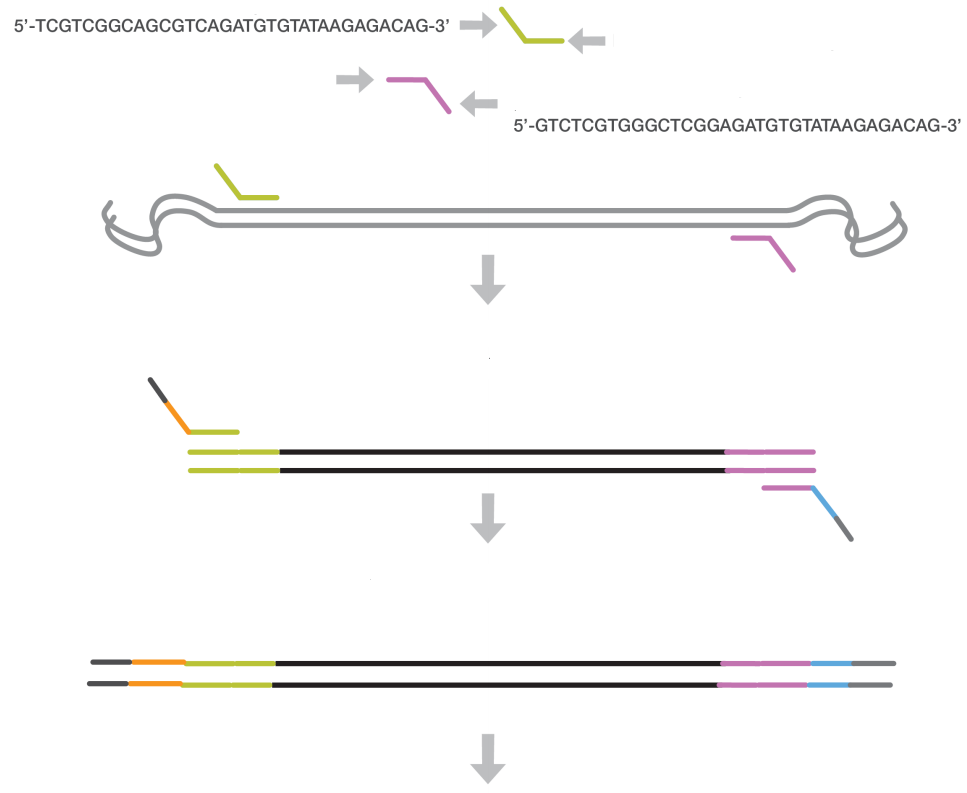
\includegraphics[width=8cm]{two_stage_pcr}
  \centering
  \caption{Двустадийная ПЦР}
  \label{img:two_stage_pcr}  
\end{figure}

Далее проводилась чистка полученныйх ампликонов от свободных праймеров и димеров с использованием AMPure XP beads (Beckman Coulter, США). Для наиболее эффективной очистки брали  20 мкл AMPure XP beads. Далее для качественной оценки ПЦР продукта был проведен электрофорез в 2\% агарозном геле. 

После того, как были выбраны накоплены необходимые вариабельные участки, шла вторая стадия ПЦР, на которой к образцам пришивались индексированные праймеры.  Для каждого образца составлялась смесь общим объемом 50 мкл, которая содержала 

\begin{itemize}
\item 5 мкл матрицы
\item 5 мкл буфера для ПЦР
\item 5 мкл dNTP
\item 1 мкл каждого из двух индексированных праймеров
\item 0,5 мкл полимеразы
\item 32,5 мкл воды
\end{itemize}

Далее проводили реакцю при следующих условиях:

\begin{enumerate}
	\item $95^{\circ}$ , 3 мин – денатурация;
	\item 8 циклов:
	\begin{itemize}
		\item $95^{\circ}$, 30 с – денатурация
		\item $55^{\circ}$, 30 с – отжиг праймеров на матрице
		\item $72^{\circ}$, 30 с – элонгация
	\end{itemize}
	\item $72^{\circ}$, 5 мин – ?
	\item $4^{\circ}$ ,  $\infty$
\end{enumerate}

Далее проводилась чистка полученныйх ампликонов от свободных праймеров и димеров с использованием AMPure XP beads. Для наиболее эффективной очистки брали  56 мкл AMPure XP beads. Далее образцы анализировались с использованием Bioanalyzer DNA 1000 chip для проверки размера полученной библиотеки (~630п.о.). 

Далее образцы смешивались в эквимолярном соотношении: рассчитывается концентрация ДНК в нМ, определенная Agilent Technologies 2100 Bioanalyzer.

\begin{equation}
\dfrac{\text{концентрация в нг/мкл}}{\text{660 г/моль \* средний размер библиотеки}}\*10^6=\text{концентрация в нМ}
\end{equation}

\vspace{\baselineskip}

Далее полученная библиотека была отсеквенирована с помощью прибора Illumina MiSeq (Illumina, США) согласно инструкциям и рекомендациям протокола производителя. 

\subsection{Секвенирование вариабельных участков V2-4-8/ V3-V6,V7-9 гена 16S рРНК с помощью секвенатора IonTorrent PGM }  \label{subsect1_2_3}

Приготовление библиотеки происходило в соответсвии с протоколом \textit{Ion} $16S^{TM}$ \textit{ Metagenomics Kit (Life Technologies, США)} (см. рис. \ref{img:workflow}). Было использовано два набора праймеров для вариабельных участков V2-4-8/ V3-V6,V7-9. 

\begin{figure}[h]
  \includegraphics[width=8cm]{workflow}
  \centering
  \caption{Алгоритм работы по протоколу Ion $16S^{TM}$ Metagenomics Kit }
  \label{img:workflow}  
\end{figure}

Для получения необходимых ампликонов была проведена ПЦР. Для кажого образца готовилась смесь, общим объемом 30 мкл, которая содержала 

\begin{itemize}
\item 15 мкл 2X Environmental Master Mix
\item 3 мкл 16S Primer Set $(10X)^{[1]}$
\item 2-12 мкл образца
\item объем воды, необходимый до 30 мкл
\end{itemize}

Далее проводили реакцю при следующих условиях:

\begin{enumerate}
	\item $95^{\circ}$ , 10 мин – денатурация;
	\item 18-25 циклов:
	\begin{itemize}
		\item $95^{\circ}$, 30 с – денатурация
		\item $58^{\circ}$, 30 с – отжиг праймеров на матрице
		\item $72^{\circ}$, 20 с – элонгация
	\end{itemize}
	\item $72^{\circ}$, 7 мин – ?
	\item $4^{\circ}$ ,  $\infty$
\end{enumerate}

Далее проводилась чистка полученныйх ампликонов от свободных праймеров и димеров с использованием AMPure XP beads.  Для наиболее эффективной очистки брали  1,8 V от образца AMPure XP beads. Далее из очещенных ампликонов готовили библиотеку для секвенирования. 
На первом этапе происходила достройка концов ампликонов, при помощи инкубации их при комнатной температуре в течение 20 минут с использованием 5X End Repair Buffer и End Repair Enzyme . Далее проводилась чистка полученныйх ампликонов от свободных праймеров и димеров с использованием AMPure XP beads. Затем были лигированы адаптеры и проведена никтрансляция. Для этого была проведена ПЦР. Для кажого образца замешивалась смесь, общим объемом 100 мкл, которая содержала 

\begin{itemize}
\item 25 мкл матрицы
\item 10 мкл 10X Ligase Buffer
\item 2 мкл Ion P1 Adapter
\item 2 мкл Ion Xpress™ Barcode X[1] 
\item 2 мкл dNTP Mix
\item 49 мкл Nuclease-free Water
\item 2 мкл DNA Ligase
\item 8 мкл Nick Repair Polymerase
\end{itemize}

Далее проводили реакцю при следующих условиях:

\begin{enumerate}
	\item $25^{\circ}$ , 15 мин;
	\item $72^{\circ}$, 5 мин;
	\item $4^{\circ}$ ,  $\infty$.
\end{enumerate}

После следовала чистка ампликонов от свободных праймеров и димеров с использованием AMPure XP beads (1,4 V). Затем измеряли концентрацию, используя Qubit, проверяли качество библиотеки на Bioanalyzer DNA HS chip. Разводили библиотеки до концентрации 100 пмоль, смешивали в эквимолярном соотношении (аналогично протоколу Illumina). Далее следовала эмульсионная ПЦР, чтобы посадить фрагментную библиотеку на специальные шарики, которые впоследствии будут нанесены на чип для секвенирования. Так как данный процесс имеет погрешность, то есть не все шарики оказываются связанными с бибилотекой, то была проведена процедура обогощения, в процессе которой мы избавились от пустых шариков. Затем следовало нанесение уже обогощенной баблиотеки на чип, и далее было проведено секвенирование.




\subsection{Shotgun-секвенирование}  \label{subsect1_2_4}
Приготовление библиотеки происходило в соответсвии с протоколом $IonXpress^{TM}$ \textit{Plus gDNA Fragment Library Preparation}.

Выделенную ДНК необходимо было поделить на фрагменты длинной 200 пар оснований. Данный этап происходил с использованием Covaris (S220 Focused-ultrasonicators). После необходимо достроить концы фрагментов, для этого была проведена инкубация при комнатной температуре с использование  \textit{5X End Repair Buffer} и  \textit{End Repair Enzyme}. Избавление от димеров и фрагментов малой длины (\~50 п.о.) происходило при чистке с использованием \textit{Agencourt AMPure XP Kit} (1,8 V). Следующим этапом было лигирование адаптеров и никтрансляция. Для этого ставилась ПЦР. Для каждого образца замешивалась смесь общим объемом 100 мкл, которую впоследствии делили на две пробирки одинакового объема для лучшего протекания реакции. Каждая пробирка содеражала 

\begin{itemize}
\item 25 мкл ДНК
\item 10 мкл 10X Ligase Buffer
\item 2 мкл Ion P1 Adapter
\item 2 мкл Ion Xpress Barcode X
\item 2 мкл dNTP Mix
\item 49 мкл Nuclease-free Water
\item 2 мкл DNA Ligase
\item 8 мкл Nick Repair Polymerase
\end{itemize}

Далее проводили реакцю при следующих условиях для одного цикла:

\begin{enumerate}
	\item $25^{\circ}$ , 15 мин;
	\item $72^{\circ}$ , 5 мин;
	\item $4^{\circ}$ ,  $\infty$.
\end{enumerate}

Далее была чистка от димеров с использованием \textit{Agencourt AMPure XP Kit}.

Так как существует большая погрешность при фрагментации и не все фрагменты получаются одинаковой длины, то очищение от фрагментов большой длины (\~100 п.о.) происходит с использование агарозного E-Gel. Данный этап работы называется size-select. Затем снова проводилась амплификация, чтобы увеличить концентрацию фрагментов с лигированными адаптерами. Для каждого образца замешивалась смесь общим объемом 130 мкл, которую впоследствии делили на две пробирки одинакового объема для лучшего протекания реакции. Каждая пробирка содеражала

\begin{itemize}
\item 100 мкл Platinum PCR SuoerMix High Fidelity
\item 5 мкл Library Amplification Primer Mix
\item 25 мкл неамплифицированной библиотеки
\end{itemize}

Далее проводили реакцю при следующих условиях для одного цикла:

\begin{enumerate}
	\item $95^{\circ}$ , 5 мин 
	\item n циклов:
	\begin{itemize}
		\item $95^{\circ}$, 15 с – денатурация
		\item $58^{\circ}$, 15 с – отжиг праймеров на матрице
		\item $70^{\circ}$, 1 мин – элонгация
	\end{itemize}
	\item $4^{\circ}$ ,  $\infty$
\end{enumerate}

Далее снова чистили библиотеки, измеряли концентрацию, используя Qubit, проверяли качество библиотеки на Bioanalyzer DNA HS chip. Разводили библиотеки до концентрации 100 пмоль, смешивали в эквимолярном соотношении (аналогично протоколу Illumina). Далее следовала эмульсионная ПЦР, чтобы посадить фрагментную библиотеку на специальные шарики, которые впоследствии будут нанесены на чип для секвенирования. Так как данный процесс имеет погрешность, то есть не все шарики оказываются связанными с бибилотекой, то была проведена процедура обогощения, в процессе которой мы избавились от пустых шариков. Затем следовало нанесение уже обогощенной баблиотеки на чип, и далее было проведено секвенирование. 


\subsection{Анализ полученных данных}  \label{subsect1_2_5}

Данные, полученые с Illumina MiSeq, были обработаны програмным обеспечением, встроенным в прибор. Для классификации вариабельных фрагментов гена 16S рРНК была использована база данных GreenGenes (http://greengenes.lbl.gov/cgi-bin/nph-index.cgi) []. 

Для реконструкции гена 16S рРНК из ридов был использован геномный сборщик IDBA-UD (ссылки). Контиги были класиффицированы с использованием онлайн-сервера RDP-Classifier (https://rdp.cme.msu.edu/classifier/classifier.jsp). 

Для визуализации данных была использована программа MEGAN5 (https://rdp.cme.msu.edu/classifier/classifier.jsp).

Риды, полученные в результате shotgun-секвенирования, были собраны SPAdes Genome Assembler [http://bioinf.spbau.ru]. Полученная сборка была проаннотирована с помощью программы Prokka []. Для визуализации метаболических путей был использован онлайн ресурс KEGG [http://www.genome.jp/kegg/pathway.html]. 


\clearpage
